\section{FSM}
\label{sec:fsm}
Wir betrachten nun etwas genauer wir unsere Konzept einer FSM zur 
Kontrollflusssteurung in C++11 umgesetzt haben, dazu gehört neben der Wahl 
der Klassenstruktur auch die Einbindung nützlicher Features von C++11 um die
Speicherverwaltung zu optimieren.


%%%%%%
\subsection{Klassenstruktur}
Zur Modellierung einer FSM haben wir ein Konzept aus einer Kontroller Klasse \texttt{FSM} und zwei abstrakten Basisklassen \texttt{State} und \texttt{Transition} überlegt. Dabei stellen die abstrakten Basisklassen nur eine standardisiertes Interface bereit und erlauben somit einen schnelle Implementation von neuen abgeleiteten Klassen.


Erst die abgeleiteten Klassen implementieren eine genau Funktionalität, wie z.B. einer Wandfolgen oder eine Transition nach einem bestimmten Ereignis. Diese Klassen sind in dem dafür vorgesehen namespace \texttt{TRAL::STATES} und \texttt{TRAL::TRANSITIONS} zu finden.

\begin{figure}[htbp] 
  \centering
     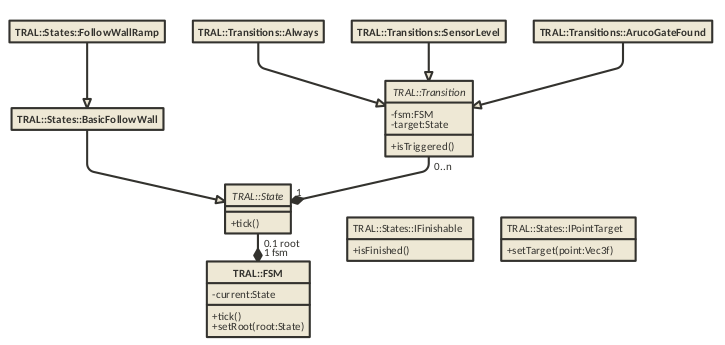
\includegraphics[width=\textwidth]{images/fsm-uml.png}
  \caption{Vereinfachtes Klassendiagram der FSM}
  \label{fig:KlassendiagramFSM}
\end{figure}

%%%%%%
\subsubsection{FSM}
Die Klasse \texttt{FSM} implementiert die komplette Kontrollflusssteuerung und kümmert sich ebenso um das Laden einer FSM die zuvor graphisch mit Umlet erstellt wurde. Ebenso hält diese Klasse immer eine aktuelle Referenz zum dem globalen \texttt{MachineState}, in dieser Klasse sind alle Sensorinformationen aufbereitet konsolidiert.

\paragraph{\texttt{FSM::tick}}

Die wichtigste Funktion diese Klasse ist die \texttt{tick} Funktion, diese wird zyklisch von der Rosnode tral-fsm aufgerufen. Dabei wird der Kontrollfluss an den aktuell aktiven State weitergeben. Wenn nun der aktive State einen neuen Ausgabe gesetzt hat und die Kontrolle wieder abgibt werden nun alle an diesen State befindlichen Transition überprüft ob diese Ausgelöst haben, sollte dies der Fall sein wird eine \texttt{transit} vollzogen.

\paragraph{\texttt{FSM::transit}}

Beim Statewechsel wird zuerst dem aktuell noch aktiven State signalisiert das der nun verlassen wird, dabei kann der State
zum Beispiel genutzte Ressourcen wieder freigeben. Darauf folgend wird dem neuen State signalisiert das dieser nun betreten wird und nötige Ressourcen belegen kann.


%%%%%%
\subsubsection{State}
Die Klasse \texttt{TRAL::State} ist eine abstrakte Basisklasse von dieser werden alle States abgeleitet, für unsere implementation wurden zum Beispiel folgende States abgeleitet:

\begin{itemize}
	\item ApproachPoint
	\item ArucoGateCenter
	\item BasisFollowWall
	\begin{itemize}
		\item FollowWall
		\item FollowWallRamp
	\end{itemize}
	\item Idle
	\item Motor
	\item Stop
\end{itemize}

Jeder instantiierbarer State muss alle virtuellen Funktion der State Klasse implementieren. Dadurch wird gewährleistet das die FSM Klasse mit jede beliegen State Implementation arbeiten kann.

Die statische Funktion \texttt{createFromJson} erlaubt ein State Instanz aus einem JSON Objekt erzeugen Als virtuelles Interface sind die Funktion \texttt{tick}, \texttt{onEnter}, \texttt{OnExit} und weitere Debug-Funktionen vorgesehen.

\texttt{onEnter} und \texttt{OnExit} signalisieren das zuvor beschriebene betreten und verlassen eines States bei der Ausführung. Die Funktion \texttt{tick} wird für den aktiven State zyklisch ausgeführt und berechnet einen neue Ausgabe. Dabei kann über den globalen \texttt{MachineState} auf die aktuellen Sensorwerte zugegriffen und die Aktoren angesteuert.


%%%%%%
\subsubsection{Transition}
Ähnlich der State Klasse fungiert die \texttt{TRAL::Transition} als abstrakte Basisklasse für alle Transitionen. Ebenso existiert auch eine statische Funktion \texttt{createFromJson} um gespeicherte Instanz aus einem JSON Objekt zu laden. 

Jede Transition gehört zu einen eindeutigen Besitzer \textit{owner} und zu einem eindeutigen Ziel \textit{target}. Sollte der \textit{owner} State aktuell aktiv sein wird jene Transition auf Auslösung, mit der Funktion \texttt{isTriggerd}, durch die FSM Instanz nach der Ausführung des States überprüft.

Für unsere Implementierung haben wir folge Transitionen abgeleitet:

\begin{itemize}
	\item Always
	\item ArucoGateFound
	\item Distance
	\item Finished
	\item SensorLevel
\end{itemize}

%%%%%%
\subsubsection{Interfaces}

Um die Übergabe von Informationen zwischen zum Beispiel einem State und einer Transtion zu gewährleisten haben wir zwei Interfaces für States verwendet. 
States die das Interface \texttt{IFinishable} einbinden können entscheiden wenn diese Abgeschlossen sind. Zum Beispiel implementiert der State \texttt{ApproachPoint} diese Interface und signalisiert die Ankunft an dem definierten Punkt.

Ebenso können States die das Interface \texttt{ApproachPoint} implementieren ein Zielpunkt gesetzt bekommen. Diese Interface wird auch zum Beispiel vom State \texttt{ApproachPoint} implementiert und erlaubt so ein verlegen des definierten Punktes bei der Ausführung.

Soll muss zum Beispiel der \textit{owner} State der \texttt{Finished} Transition das dazugehörige Interface implementieren, sollte dies nicht der Fall sein kommt es zu einem Laufzeitfehler während der Ausführung.
